\section{Ingestion-Service}
\label{sec:entw-ingestion}

Der Ingestion-Service hat die Aufgabe eine Ingestion für eine Datenquelle durchzuführen.
Dazu gehören das Laden der Daten in ein DataFrame, die Deltaberechnung und das Speichern.
Das meiste davon wird jedoch nicht von dem Service selbst, sondern auf dem Spark Cluster gemacht.
Der Service führt die Vorbereitung und das Deplyoment des Jobs auf dem Cluster aus.

Der Ingestion-Service wartet auf die Nachricht zur Ausführung einer Ingestion, mit der Id der DatasourceDefinition.
Als erstes wird dann geprüft, ob bereits eine Ingestion der Datenquelle aktiv ist.
Falls das nicht der Fall ist, wird ein neuer Prozess gestartet, indem die Ingestion ausgeführt wird.
Auf diese Art können mehrer Ingestion von verschiedenen Quellen parallel bearbeitet werden.

Der Ablauf einer einzelnen Ingestion kann unabhängig vom Lese- und Schreib-Typ in einem allgemeinen Ablauf abgebildet werden.
Als erstes wird die Ingestion vorbereitet.
Hier werden die Plugins installiert und eine SparkSession erstellt.
Im nächsten Schritt werden die Daten aus der Quelle geladen.
Wenn es sich dabei um Ändeurngsdaten aus einer Updatequelle handelt, können diese direkt in den entsprechenden Zieldatensatz eingepflegt werden.
Ist das nicht der Fall, foglt eine Entscheidung, ob Änderungsdaten berechnet werden müssen.
Es gelten die folgenden zwei Regeln: \begin{itemize}
    \item der Speicher-Typ ist Delta
    \item es ist nicht die erste Ingestion dieser Datenquelle
\end{itemize}
Wurden Änderungsdaten berechnet, werden diese eingepflegt und ansonsten einfach gespeichert.
Handelt es sich nicht um einen benutzerdefinierten Speicher, werden die alten Daten mit den neuen überschrieben.

\begin{figure}
    \centering
    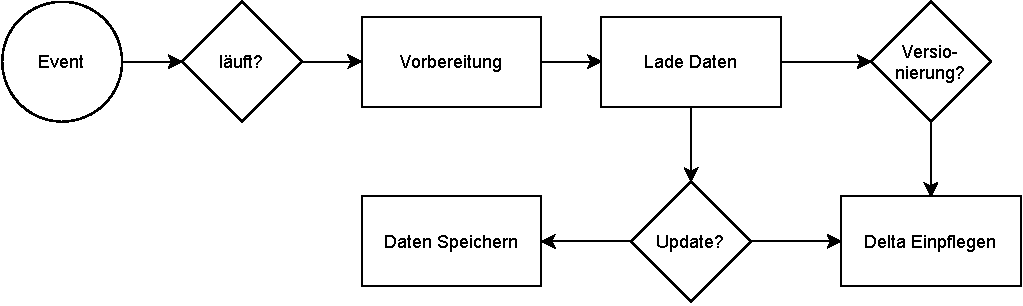
\includegraphics[width=\textwidth]{Grafiken/Entwicklung-Ingestion-Ablauf.pdf}
    \caption{Ablauf einer Ingestion}
    \label{fig:ingestion-ablauf}
\end{figure}